%%%%%%%%%%%%%%%%%%%%%%%%%%%%%%%%%%%%%%%%%%%%%%%%%%%%%%%%%%%%%%%%%%%%%%%%%%%%%%%%
% reconstruction.tex:
%%%%%%%%%%%%%%%%%%%%%%%%%%%%%%%%%%%%%%%%%%%%%%%%%%%%%%%%%%%%%%%%%%%%%%%%%%%%%%%%
\chapter{ Particle Identification and Event Reconstruction}
\label{reconstruction_and Particle_ID_chapter}
%%%%%%%%%%%%%%%%%%%%%%%%%%%%%%%%%%%%%%%%%%%%%%%%%%%%%%%%%%%%%%%%%%%%%%%%%%%%%%%%
\section{Particle Reconstruction}
Reconstruction is the operation of constructing physics quantities from raw data collected in the experiment. It is a software process whose objective is data reduction to higher-level objects use for data analysis.
An event observed by the CMS detector is reconstructed using information from the different sub-detectors. This information represents the raw data from the DAQ which is in a format called digitised hits or \textit{digis}. A local reconstruction is performed with the output from these reconstruction units called \textit{RecHits}. The local reconstruction algorithm search for pixel or strips with a signal exceeding a threshold  and use these as seeds for clusters. RecHits are typically position measurements~(from times or clusters of strips or pixels) in tracking type detectors~(Muon and Tracker systems) and energy deposits or hits from Calorimetry systems. For example in the Muon Cathode Strip Chambers~(CSCs),local reconstruction provides position and time of arrival of muon hit from the distribution of charge induced on the cathod strips. For  the case of the Electromagnetic Calorimeter~(ECAL) and Hadronic Calorimeter~(HCAL), local reconstruction identifies, the position, time of arrival and energy of localised electromagnetic and hadronic energy depositions respectively. The typical software package for local reconstruction is label as RecoLocalTracker as in the case of tracks indicating only local modules of the sub-detector have been used. Global reconstruction takes these rechits as input to produced higher-level objects like charge particle tracks. This is where information from different modules in the same sub-detectors are combined. Clustering, tracking and fitting algorithms are used at this stage. For example, in ECAL and HCAL, global reconstruction provides a Calorimetric Tower~(CaloTower) links matching clusters in ECAL and HCAL   to produced a projective tower in the calorimetric system.  These towers have a definite position in $(\eta, \phi)$ plane and are used as basis for Jet reconstruction as described later in the sub-sections. In the Tracker, global reconstruction uses tracker hits and track segments and use the seeds for Kalman fitter which builds trajectories  with a $\chi^{2}$ cut applied to reject hits unlikely to be associated with tracks. The typical software packaged is label RecoTracker again as in the case of full charge particle tracks. The final reconstruction combined reconstructed objects from individual sub-detectors to produced  higher-level reconstructed objects  suitable for high-level triggering or physics analysis. Further selection requirements may be further applied until the final physics objects such as electron, photon or jet belonging to the event is fully reconstructed.
%%%%%%%%%%%%%%%%%%%%%%%%%%%%%%%%%%%%%%%%%%%%%%
\subsection{Supercluster Reconstruction}
The basis of all object reconstruction is the supercluster or basic cluster. Electromagnetic showers of photons and electrons are deposited in several crystals. Usually about 94\%~(97\%) of the incident energy is deposited in a $3\times3$~($5\times5$) matrix crystals in the $(\eta, \phi)$ plane. The presence of $3.8$~T magnetic field, material in front of the calorimeter causes bremssrahlung electrons and converted photons to deposit their energy in calorimeter in the form of small clusters spread in $\phi$.  This energy is recovered using clustering algorithms  where by starting with a seed crystal containing the maximum  of energy, superclusters~(clusters of cluster) are build within a narrow window in $\eta$ by is summing  the crystal energy along the $\phi$ which is the direction of energy spread due to the magnetic field. Figure \ref{fig:CLUSTER} shows a simple picture how these super clusters are build.
\begin{center}
%\begin{figure}
\centering
\mbox{
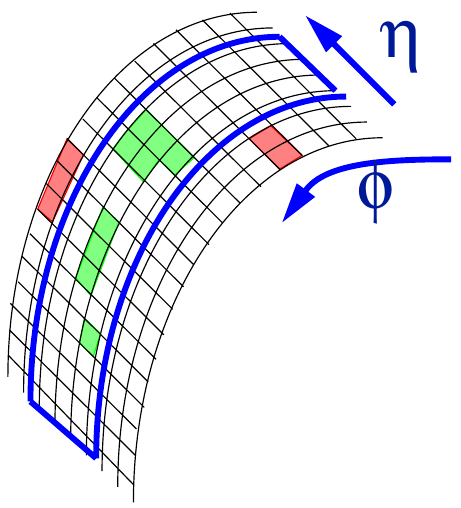
\includegraphics[scale=0.5]{THESISPLOTS/ECAL_CLustering.png}\quad
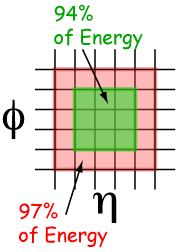
\includegraphics[scale=0.8]{THESISPLOTS/BasicCluster.png}}
\captionof{figure}{Superclustering algorithm in ECAL for both hybrid~(EB) and island~(EE) clustering algorithms.} \label{fig:CLUSTER}
%\end{figure}
\end{center}

 There are two major clustering algorithms used:
\begin{itemize}
\item \textbf{Hybrid Superclusters:} This algorithm is used to make super-clusters in the barrel~(EB). It takes advantage of the $\eta - \phi$ geometry of barrel crystals by taking a fixed 3 or 5 crystals in $\eta$ and dynamically search and sum separate crystals energy along $\phi$. The Hybrid algorithm takes advantage of our knowledge of the lateral shower shape along the $\eta$ direction. The supercluster is made of basic clusters.
The figure \ref{fig:HYBRID} shows an example of how the hybrid clustering algorithm performs clustering.
\begin{center}
%\begin{figure}
\centering
\mbox{
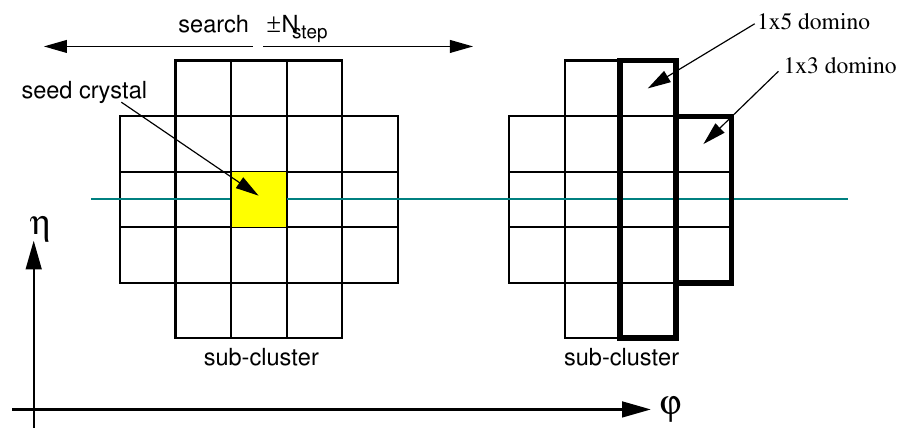
\includegraphics[scale=0.5]{THESISPLOTS/Hybrid_Clustering_ECAL.png}}
\captionof{figure}{Superclustering in ECAL for hybrid clustering algorithm in barrel.} \label{fig:HYBRID}
%\end{figure}
\end{center}

\item \textbf{Island Basic cluster or Superclusters:} After Local reconstruction leading to the production of \textit{EcalRecHits}, the island algorithm is applied in both barrel and endcap~(EE)to produce superclusters. This algorithm begins by finding the seed crystal with a local energy maximum above a certain threshold. from the seed position, adjacent crystals are examined starting fist along $\phi$ and then in $\eta$ adding crystal energy to cluster until a crystal belonging to another cluster or crystal that has no readout is reached. For each crystal to be added to the cluster,  the crystal must contain a rechit with positive energy, the crystal has not been assigned to another cluster and the previous crystal added in the same direction has higher energy. These non-overlapping clusters are then made into superclusters. A search is performed for the most energetic cluster and then collect all the other narrow window clusters in $\eta$ and wide window in $\phi$. The figure in \ref{fig:ISLAND} provides a pictorial view of how the island algorithm works.
\begin{center}
%\begin{figure}
\centering
\mbox{
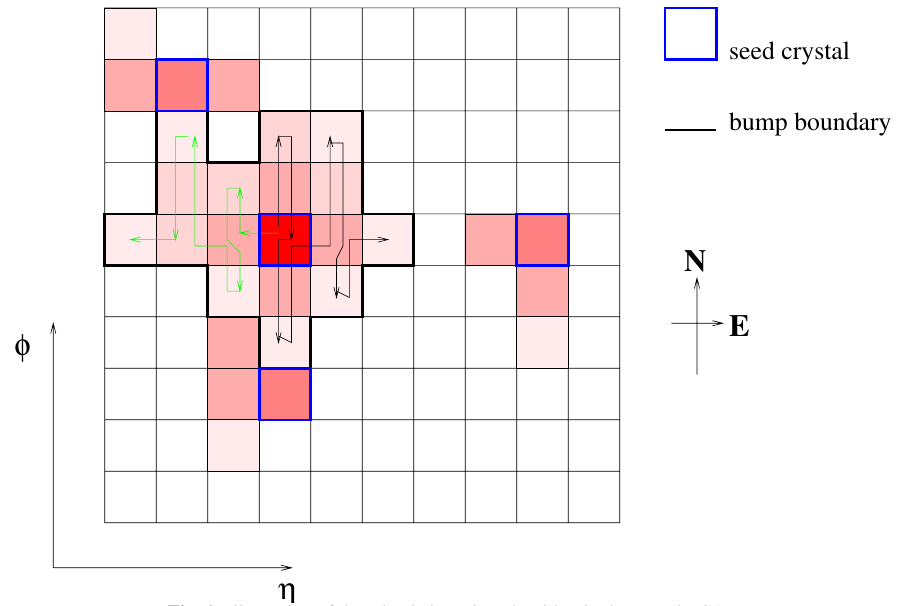
\includegraphics[scale=0.5]{/home/tensr/Documents/TEN-HEP-PHD-THESIS/PHD_THESIS/PHD/THESISPLOTS/ISLAND_Clustering_ECAL.png}
}
\captionof{figure}{Superclustering in ECAL for Island clustering algorithm in barrel.} \label{fig:ISLAND}
%\end{figure}
\end{center}
 
\end{itemize} 

\subsection{Vertex and Track Reconstruction}
The reconstruction of track candidates of a charge objects such as an electron begins by selecting an initial parameter which a pair or triplet of hits constraint by the interaction region or a given beam spot in the pixel detector.  This if followed by the search of other pairs of hits in pairs of tracker layers as well as hit pairs in the strips or strips an pixels  to allow for reconstruction of vertices beyond the pixel volume. To prevent the combination factor and reduce fake rates when using the Combinatorial Track Finder~(CTF), hits are selected in a small restricted region in $\phi$  compatible with a super-cluster in the ECAL. This seeding strategy is known is \textit{tracker-driven}. Another  powerful approach is to start with  the ECAL super-cluster and match the seed super-cluster hits back towards hit in the tracker particular the pixel. It is term \textit{ECAL-driven} seeding and this super-cluster-driven pixel seed finding presents advantage for comparable reconstruction efficiency and increasing the purity by reducing the presence of fake tracks in the sample of candidate tracks. This is particularly useful for electron reconstruction and is used by the Higher Level Trigger~(HLT) for tagging primary electron-like objects. \newline
In selecting the seed cluster, the cluster which initiates the bremsstrahlung recovery procedure, this seed is required to have a minimum Transverse Energy~($E_{T}$)  of  1 GeV is $E_{T} > 1$~ GeV. This requirement allows the reconstruction of electron super-cluster for with low Transverse Momentum~($p_{T}$). In a study using back-to-back $e^{+}e^{-}$ events, a supercluster reconstruction efficiency of of about 93\%  is achieved for electron $p^{e}_{T}  = 10$~ GeV/c when $E^{seed}_{T} > 1$ GeV.
Using this seed cluster, the hits in the pixel layer are predicted by the propagation of an energy weighted mean position of the super-cluster backward through the magnetic field under the charge hypothesis( positive or negatively charged particle) towards the pixel detectors. A first compatible hit is looked for in the inner most~(barrel) of the pixel detector within a loose $\Delta\phi$ window adapted to the uncertainty  of $\phi$ measurement of the super-cluster ($\phi_{SC}$) and loose $\Delta z$ interval adapted to the spread of the interaction vertices. In case no hit is found in the innermost pixel layer, the first hit is looked for in the netx-to-innermost layer. Once a compatible hit is found, a new  estimate of the $z_{0}$ on the $z$ coordinate of the primary track vertex is calculated by combining the pixel hit found and the information from the calorimeters in the $RZ$ plane. Using this predicted trajectory, we propagate once more to look for the second pixel hit in the next pixel layer(s). 

Starting from this seed ( pair hits), a trajectory is created. This trajectory creating begins be first searching for the next silicon layer hits, then extrapolation is performed using a model based on the non-gausssian nature of energy losses by Bethe and Heitler, then Gaussian Sum Filter ~(GSF) algorithm is used to perform a fit on the track. This procedure is repeated untill the last trackers layers  unless no hit if found on the subsequent layers. If many hits a found on a compatible layer, many candidate tracks are build in parallel and using the $\chi^{2}$ from the GSF fit, the best two GSF track candidates with the smallest  $\chi^{2}$ is selected and kept. A minimum of five hits is required to create a track. The difference between electrons and photons at this stage is that photons because they are neutral have no pixel hits and as a result have no reconstructed tracks. Thus, from the ECAL driven track reconstruction, super-clusters with no pixel matched seeds fall into the photon candidate sample collection. However, 50\% of the time photons due to the tracker material will convert into $e^{+}e^{-}$ conversion pairs. These are known as \textit{converted photons}. These converted photons are usually low $p_{T}$ photons and don't always travel to the ECAL but those that do and if happen to arrive late can be candidates for clear signal of physics beyond the SM. Because electrons have a GSF tracks , they are normally referred to as GSF electrons.   Using the selected GSF tracks, important particle kinematic information such as the vertex pseudo-rapidity~($\eta$), the track $p_{T}$ and the vertex $\phi$ coordinate are well measured with good resolution.
\newline
The primary interaction vertex in an event is reconstructed from a collection of tracks. A group of tracks in clusters based on the $z$ coordinate position of their track with respect to the point of closest approach to the beamline. The track clusters, as previously mentioned are fitted with and adaptive vertex fitter and the tracks are assigned  weights between 0 and 1 based on their closeness in proximity to the common vertex. This ensures a dependence on the primary vertex resolution to the number of tracks used in the fitting and $p_{T}$. This primary vertex resolution dependence on the number of tracks is studied using tracks in an event with just one vertex while for $p_{T}$, the resolution is studied for a number of tracks with different average $p_{T}$ of tracks in the vertex. It is important to recall that tracks can only be reconstructed up to $|\eta| < 2.5$  which defines the tracker volume, beyond which these objects are assumed to have no tracks.
%%%%%%%%%%%%%%%%%%%%%%%%%%%%%%%%%%%%%%%%%%%%%%%%%%%%%%%%%%%%%%%%%%%%
\subsection{Photon or Electron Identification}
Electron and photon identification depends of the ability to reject minimum biased events, underlying events or Pile Up~(PU) produced from multiple proton-proton interactions, electrons embedded in hadronic showers or Jets and anomalous events. 
Pre-selections are applied at the level of track seeding and clusters so as to reject tracks from underlying or low energy proton-proton collision events called Pile Up~(PU).
Based on kinematic and nature of electromagnetic showers in the ECAL, some variables have been developed and their performance studied for optimal identification and isolation of electrons and photons. This is in compatibility with the fact that the two electron reconstruction algorithms compliment each other in specific $p_{T}$ range. The tracker seed driven algorithm is more suitable for low $p_{T}$ electrons as well as better performance for electrons inside jets while  ECAL seed driven algorithm which selects seeding clusters with transverse energy $E_{T} > 1$~GeV is optimised for isolated  electrons
$p_{T} > 10~GeV/c$  up to $p_{T}$ relevant for the mass of $Z$ or $W$ bosons.
\newline
The goal of the ECAL is to obtain the best estimate of energy deposited by an electron or photon in the ECAL, $E_{e/\gamma}$. This from the detector point of view, the energy deposit is given as:

\begin{equation}\label{eEnergy}
E_{e/\gamma} = F_{e/\gamma} \cdot [ G \cdot \sum_{i} S_{i}(t) \cdot C_{i} \cdot A_{i} ]
\end{equation}
where $A_{i}$ is the signal amplitude in ADC counts, $C_{i}$ is the inter-calibration coefficient,  $S_{i}(t)$ is the time-dependent corrections  for response variable usually obtain from laser, $G$ is the global scale calibration allowing one to move form energy in ADC counts to GeV and $F_{e/\gamma}$ is the particle energy corrections for geometric, clustering and other effects. The sum is over all the crystals belonging to the photon or electron super-cluster. In order to measure and reconstruct the true energy of the detected particle, energy corrections depending on $\eta$ such as $F_{e/\gamma}$ are applied at the level of super-cluster reconstruction to account for detector effects hence better identification of particles, in this case electrons and photons. Figure \ref{fig:EnergyCorr} shows energy scale and resolution obtained when these energy corrections are applied compared with when no corrections are applied. Figure \ref{fig:SCEnergyCorr}, shows the scenario for applying these corrections at the level of super-cluster reconstruction which at this stage are only electromagnetic objects.
\begin{center}
\centering
\mbox{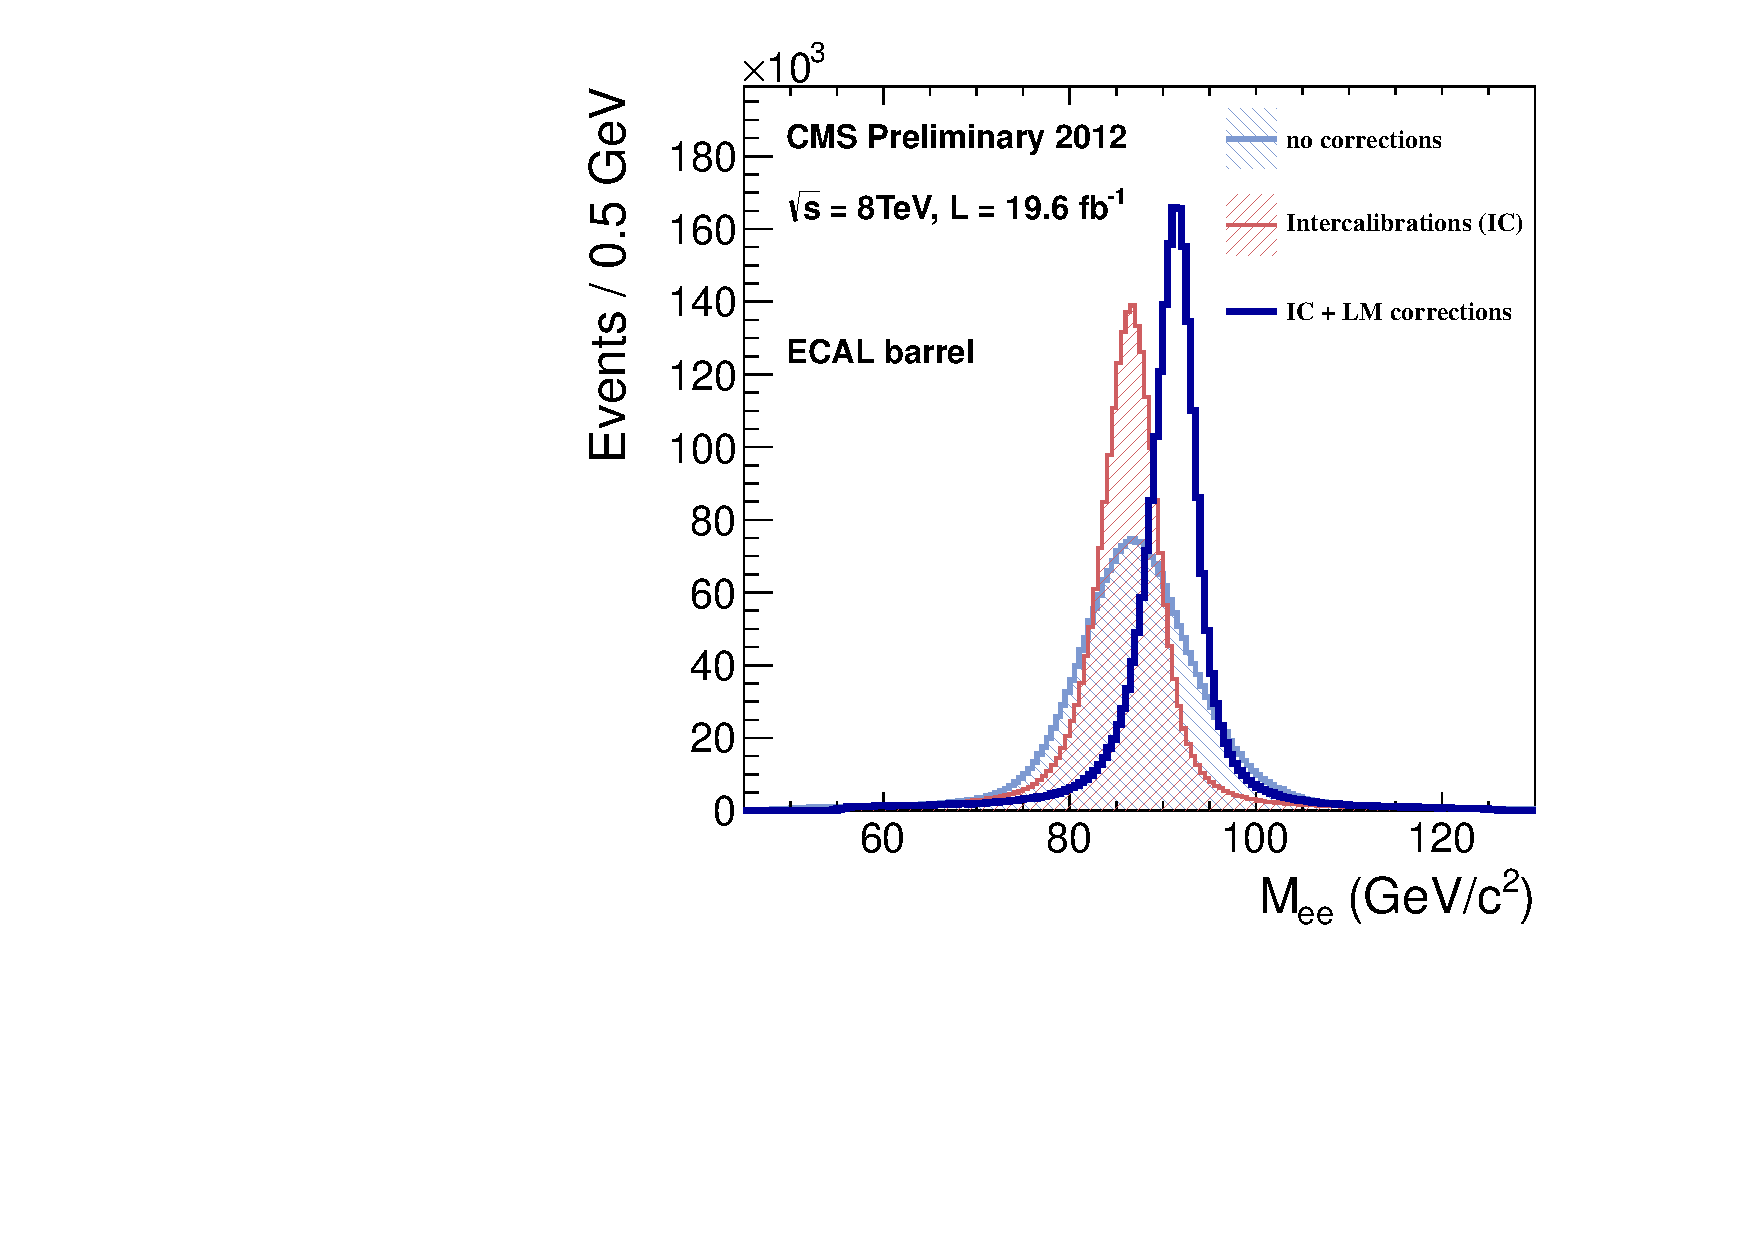
\includegraphics[height=2.0in]{THESISPLOTS/propaganda_noIC_noLaser-regrCorr_ele-EB.pdf} \quad 
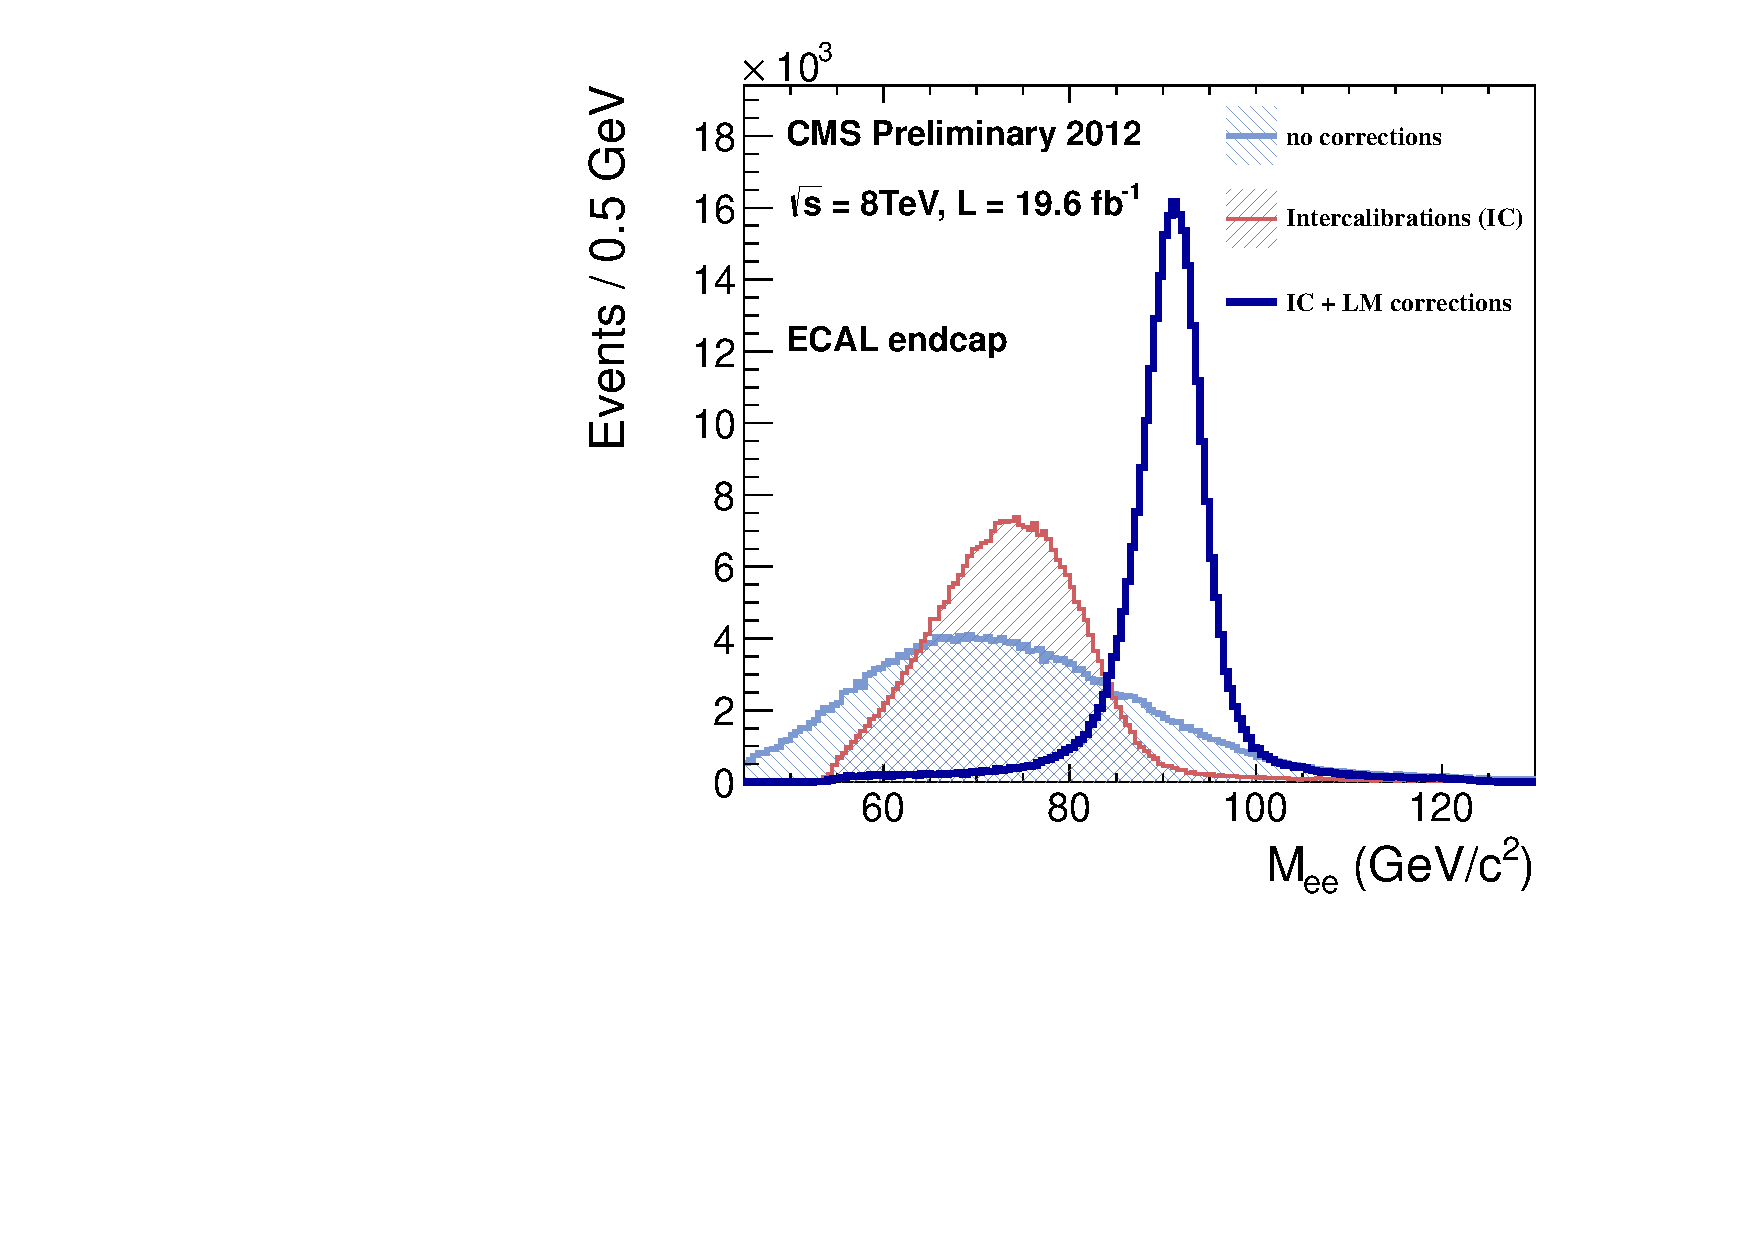
\includegraphics[height=2.0in]{THESISPLOTS/propaganda_noIC_noLaser-regrCorr_ele-EE.pdf} }
\captionof{figure}{$Z\rightarrow e^{+}e^{-}$  mass plot showing resolution and energy scale that is obtained from applying energy scale corrections to account for intrinsic spread in crystal and photo-detector response and time-dependent corrections to compensate for channel response loss for EB~(right) and EE~(left)}
\label{fig:EnergyCorr}
\end{center}

\begin{center}
\centering
\mbox{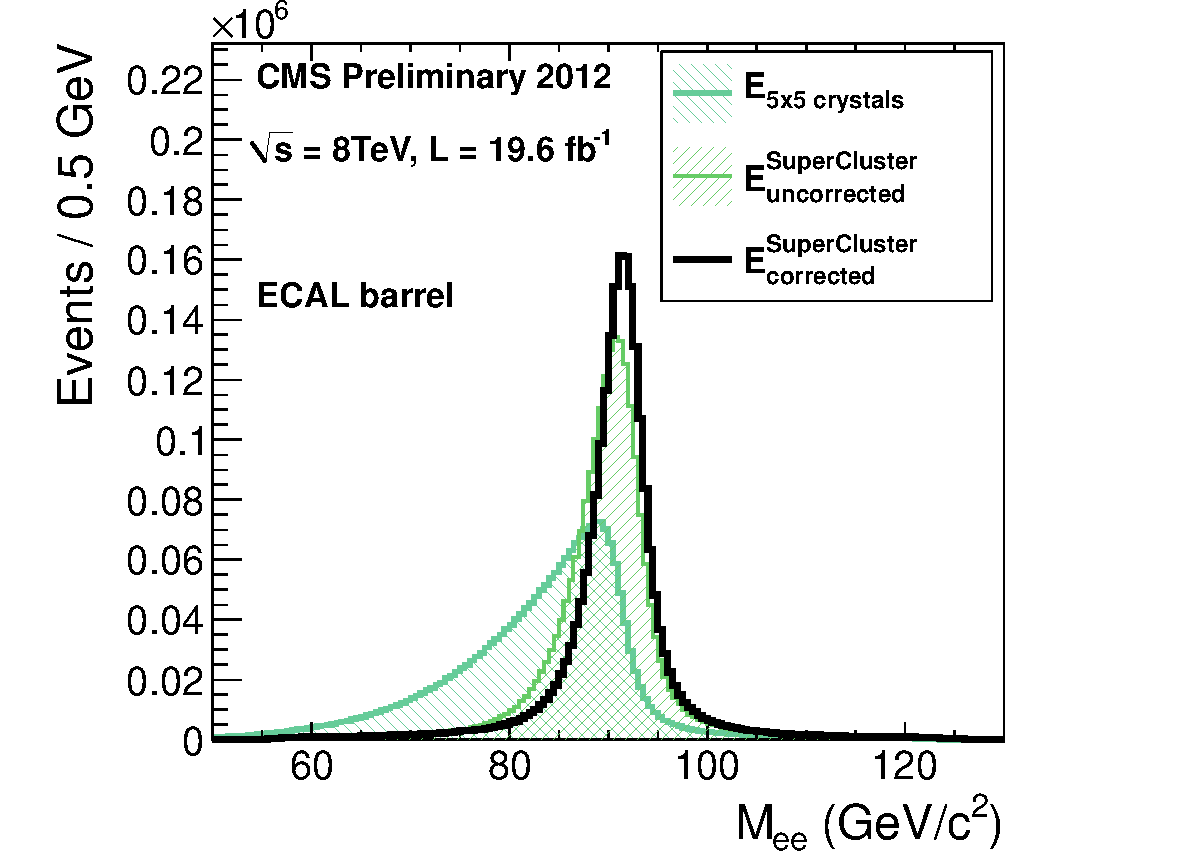
\includegraphics[height=2.0in]{THESISPLOTS/E_corr-EB.pdf} \quad 
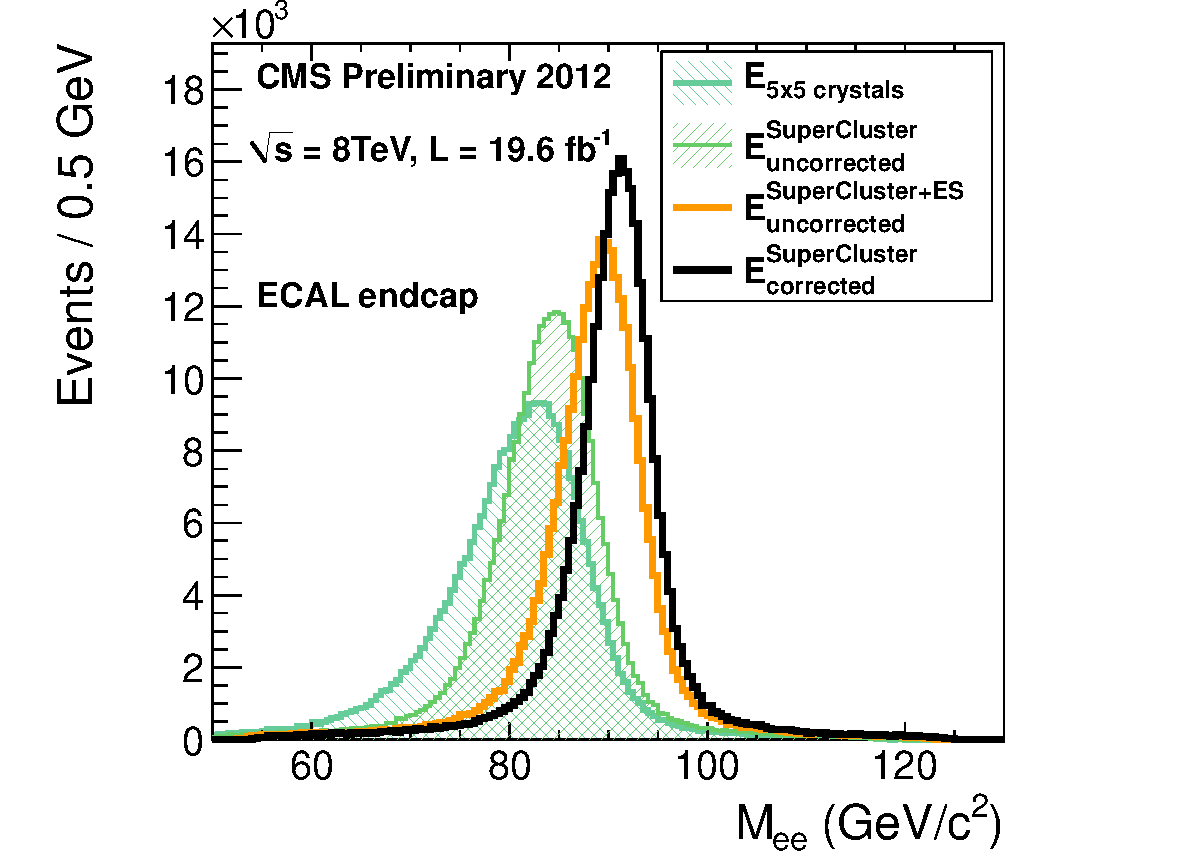
\includegraphics[height=2.0in]{THESISPLOTS/E_corr-EE.pdf} }
\captionof{figure}{Super-clusters showing resolution and energy scale that is obtained from applying energy scale corrections for EB~(right) and EE~(left)}
\label{fig:SCEnergyCorr}
\end{center}

With these electron or photon candidates, further selections using variables constructed from information on the spread of the electromagnetic shower in $\eta$ and $\phi$, the ratio of the energy deposited in ECAL and HCAL, the track $\PT$ and  ECAL $\ET$ to further identify photons and electrons.  Pre-electron candidates based on cut elections such as minimum transverse energy, $E_{T} > 4$~ GeV, $\eta$ and $\phi$ geometrical matching; $\Delta Eta < 0.02$, $\Delta \phi < 0.1$  and a cut on Ratio of hadronic to electromagnetic energy cluster: $H/E < 0.2$ is enough to suit physics analysis, however, additional elections and identification criteria are added depending on the purpose of the particular analysis to fully defined an electron or photon.
These identifications and isolation criteria can also be categorised in terms of flavours as being very loose~(VL), loose~(L), medium ~(M) and tight~(T).
The typical variables used for electron and photon identification are defined as follows:
\begin{itemize}
\item Ratio of energy of HCAL behind super cluster to super cluster energy: $H/E$
\item Energy momentum matching variables between energy of the super cluster  or of the super cluster seed and electron track  measured momentum  at the vertex or  at the calorimeter: $E/p_{in}$, $E_{seed}/p_{in}$, $E_{seed}/p_{out}$
\item Geometrical matching between the electron track parameters at the vertex  extrapolated  to the super cluster  and the measured  super cluster position: $\Delta \eta_{in}$, $\Delta \phi_{in}$.
\item Calorimeter shower shape  variables: the width of  the ECAL cluster  along the $\eta$  direction  computed  for all  the crystals  in the $5\times 5$  block of crystals centered  on the highest energy crystal  of the seed cluster ,$\sigma_{i\eta,i\eta}$ and the ratios of the energy sums over $3\times 3$ and $5\times 5$ matrices centered  on the highest energy  crystal of  the seed cluster: $R_{9} = E_{3\times3}/E_{5\times 5}$ or $R_{9} = \sum E_{9}/\sum E_{Supercluster}$. This $R_{9}$ variable makes a good separation between  unconverted photons~(energy not spread in tracker) and converted photons~(energy spread by B-field before reaching ECAL).
\item Bremsstrahlung fraction: (track momentum at vertex -  track momentum at  ECAL)/ track momentum at vertex.
\item 1/E(Super cluster) - 1/p(track at vertex)
\end{itemize}

Due to the very high photon conversion rate s as a result of the tracker material in front of the ECAL  cuts like: 
\begin{itemize}
\item  Calorimeter shower shape:$R_{9}$
\item Impact parameter: $d0$, minimum separation of the electron track computed with respect to the  reconstruction vertex.
\item Missing Hits: Number of cross layers  without a compatible hits in the back-propagation of the track to the beam-line.
\end{itemize}
 Isolation variables in addition to the identification variables are used to improve on the performance of identification. Below are the following isolation variables as defined and used by the CMS:
\paragraph*{ Electron Photon Isolation} 
 \begin{itemize}
 \item Tracker Isolation: sum of $p_{T}$ of tracks  with $p_{T} > 0.7~GeV/c$ and maximum distance to the vertex  of 0.2~cm in  a cone of 0.3 with an inner veto cone of 0.04.
 \item ECAL Isolation: sum of energy  of ECAL RecHits with a Jurassic footprint removal ~(Jurassic width of about 1.5 crystals) in a cone  of 0.4  with veto cone of 3 crystals. A RecHit noise cut of 0.08~GeV in energy~(E) in barrel and 0.1~GeV in transverse energy~($E_{T}$) in the endcap is applied.
 \item HCAL Isolation: sum of HCAL Calorimeter Towers in a 0.4 cone with a 0.15 veto cone.
 \end{itemize}
In general the major difference between an electron and a photon as identified by the CMS detector is that electrons which have no pixel strip hits are automatically  classified as photon candidates and further isolation and shower shape variables are used to arrive at the ultimate photon as required by a given analysis.
 Table \ref{tab:EGammaID} shows the Simple Cut-based selection criteria variables and cut thresholds used to identify electrons and photons in the CMS detector.

\paragraph*{Particle Flow Algorithm} \mbox{}\\
An alternative criteria for reconstructing and identifying physics objects in the CMS detector which is now widely acceptable is the \textit{particle flow}~(PF) algorithm.

The particle flow algorithm takes into consideration  information from every sub-detectors like the tracker, ECAL, HCAL and muon section before identifying a particular physics objects.
The goal of this algorithm is to reconstruct higher  level physics objects  like Jets, missing transverse energy~(MET),  and the identification of tau~($\tau$) and b-jets by making use of the content of these objects in terms of more fundamental objects like electrons and photons or super clusters and tracks.
The algorithm constitutes of steps like calorimeter clustering,  tracking and extrapolation to calorimeters, muon identification, electron pre-identification, linking of topological elements and finally particle identification and reconstruction. The result is a list of reconstructed particles consisting of photon, charge hadron, neutral hadron, muon and electron. From this list high level objects such as jets, MET and taus can be reconstructed.
In the case of electrons reconstructed using the PF algorithm, tracks, electron energy seeds, 4-momentum, super cluster energy calibration, Bremsstrahlung tracks are used as base objects to reconstruct the entire electron. The PF is very useful in MET reconstruction where information about all the particles making up a single event is necessary to calculate MET.

\begin{center}
\centering
 %\setlength{\abovecaptionskip}{0pt}
  %\setlength{\belowcaptionskip}{10pt}
 % \topcaption{GMSB,GGM Phenomenology and Relevant final states}
\begin{tabular}{|l|l|p{3.2cm}|p{3.9cm}|}
  \hline \hline
  \multicolumn{3}{|c|}{\bfseries{Simple Cut Based Electron Photon Identification}} \\
  \hline \hline
  \bfseries{ID Variable} & \bfseries{Electron} & \bfseries{Photon} \\
   \hline \hline 
  $H/E$ & 0.05(EB), 0.10(EE)  & 0.05 \\
  \hline
  $|\Delta \eta_{in}|$ & 0.005(EB), 0.007(EE)  & 0.015(EB)  \\
  \hline
   $|\Delta \phi_{in}|$ & 0.09(EB), 0.09(EE)  & N/A \\ \hline
   $\sigma_{i\eta i\eta}$ & 0.01(EB), 0.03(EE) & 0.011(EB), 0.03(EE)  \\
   \hline
   Pixel Veto & No & Yes \\
   \hline
   $|d0|(vertex)$ & 0.02(EB), 0.02(EE) &  Veto \\
   \hline
    $|dZ|(vertex)$ & 0.1(EB), 0.1(EE) & 0.02~(cm)(Veto) \\
    \hline
     $|1/E - 1/p|$ & 0.05(EB), 0.05(EE) & N/A \\
     \hline
     PF isolation / $p_{T}$ (cone dR=0.3) & 0.15(EB),0.10(EE) &  N/A \\
     \hline
     ECAL Isolation & same  & $4.2 + 0.006*E^{\gamma}_{T} + 0.183*\rho$(EB) \\
     \hline
     HCAL Isolation & same & $2.2 + 0.0025*E^{\gamma}_{T} + 0.062*\rho$ \\
     \hline
     TRACK Isolation & same  & $2.0 + 0.001*E^{\gamma}_{T} + 0.0167*\rho$ \\
     \hline
     Rho corrected PF photon isolation & N/A & $1.3 + 0.005*p^{\gamma}_{T}$(EB) \\     
     
   \hline  \hline
  \end{tabular}
   \captionof{table}{ Simple Cut-Based criteria for High energy electron and photon identification in CMS}
 \label{tab:EgammaID} % for use in \ref{table1} if you want to refer to the table number
 \end{center}
%\end{table}


\subsection{Muon Reconstruction}
%%%%%%%%%%%%%%%%%%%%%%%%%%%%%%%%%%%%%%%%%%%%%%%%%%%%%%%%%%%%%%%%%%%
The are three different types of muons reconstructed using the muon system detection all making up one huge collection of muons. They are Stand-alone, Global and  Tracker Muons.
Reconstructed hit positions within each DT and CSC  are matched to form "segments" which are then collected and matched to generate seeds used as starting point for actual track fit of DT, CSC, and RPC hits. The resulting product of the fit in the muon spectrometer is a "stand-alone muon". "Global muons are formed when these stand-alone muon tracks and matched to tracker tracks in the tracker while "tracker muons" are muon objects reconstructed starting form silicon tracker tracks compatible with segments in the muon chambers. Using muon isolation variables defined using the calorimeter and tracker tracks, a collection of muon objects is identified in CMS. Thus is summary, stand-alone muons contain only hit position information from the muon chambers, global muons contain this information in addition to tracker information while Tracker muons are muons reconstructed starting with information from the inner tracker which is matched with calorimeter and muon chamber information. Using the beam spot as a constraint ensures that muons produced from proton-proton collision are distinguished from those produce from cosmic rays known as \textit{cosmic muons} or from beam splash/gas 150~m upstream proton beam dump known as \textit{beam Halos}. The 2~T \textbf{B}-field with a multi-stage flux-return yoke shields the muon detectors from hadrons ensuring  that the measured  particles can be identified as minimum ionizing muons. The barrel muon detector  consists of 4 stations forming concentric cylinders $|\eta| < 1.2$ around the beam line while the endcaps system consists of 468 cathode strip chambers~(CSC) arranged in groups as 72~ME1/1, 72~ME1/2, 72~ME1/3, 36~ME2/1, 72~ME2/2, 36~ME3/1, 72~ME3/2and 36~ME4/1 and the 72~ME4/2. A muon in pseudo-rapidity range of $1.2 < |\eta| < 2.4 $ crosses a total of 4 CSCs. Muons in the encaps-barrel overlap region;  $0.9 < |\eta| < 1.2 $ are detected by both the barrel drift tubes~(DT) and endcaps CSCs while in bother barrel and endcaps RPSc are used for triggering. RPCs are capable of tagging the time of an ionizing event in a much shorter time than the 25~ns between 2 consecutive LHC Bunch Crossings as a result triggering based on RPC can be used  to unambiguously identify the relevant Bunch Crossing  to which a muon track is associated even in the presence of high rate and background  expected in the LHC.
\paragraph*{Cosmic and Halo Muons}\mbox{}\\
Muons produced centrally or from proton-proton collision are reconstructed a bit different from other muons. Halo muons originating from machine-induced particles travelling along the beam line and cosmic muons originating from cosmic rays require global information in order to distinguish them from centrally produced muons. Both cosmic and halo muons are considered to be background muons in most physics analysis. The stand-alone muon reconstruction software suited from reconstructed muons from proton-proton collision assumes these muons to be moving radially outward in seen in figure \ref{fig:cmsSLICE} while cosmic muons originate from the outside of the CMS detector and can traverse only a small part of a detector depending on its energy and direction.
Figure \ref{fig:Muons} show an illustration of different trajectories for the different types of muons. 

\begin{center}
\centering
\mbox{
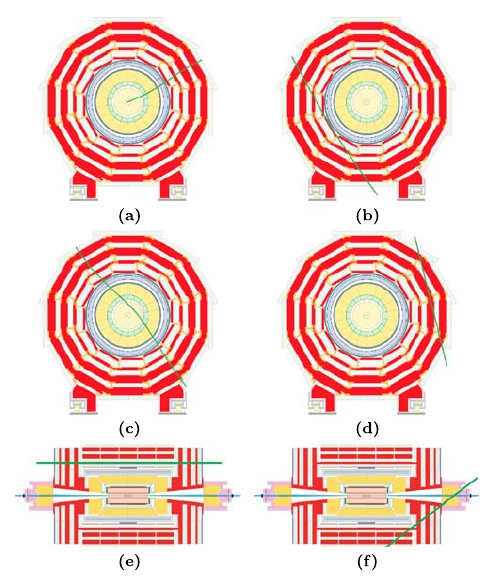
\includegraphics[height=4.0in]{/home/tensr/Documents/TEN-HEP-PHD-THESIS/PHD_THESIS/PHD/THESISPLOTS/Cosmic_Halo_Muons.png} }
\captionof{figure}{Illustration of the differences between proton-proton collision muons, cosmic and halo muons. (a) Muons from collision propagating from the center and moving outwards in a well defined pattern, (b) Cosmic muons penetrating the detector and leaving signals in opposite hemispheres of the muon system, (c) Cosmic muons leaving signals in the tracker and opposite hemispheres, (d) cosmic muons entering and leaving the detector without passing through the muon detector layers, (e) beam halo muons penetrating the detector and leaving signals in the endcaps and (f) Cosmic muons entering the detector through the endcap and leaving through the barrel and which can happen in a vice-versa manner. }
\label{fig:Muons}
\end{center}

A new stand-alone and global muon reconstruction software with the assumption that muons originate from outside the CMS detector and according to the properties of cosmic and halo muons has been optimised to reconstruct and identify both cosmic and halo muons which are used studies involving calibration and aligning the muon detectors.
\subsection{Jet Reconstruction}
%%%%%%%%%%%%%%%%%%%%%%%%%%%%%%%%%%%%%%%%%%%%%%%%%%%%%%%%%%%%%%%%%%%%%%%
Jets are experimental signatures of quarks and gluons produced in high energetic processes such as hard partons scattering in proton-proton collisions or gluon radiation processes.
CMS reconstructs four types of jets which each combine individual contributions from sub-detectors  to form inputs to a jet clustering algorithm. The four types of jets include Calorimeter jets, Jet-Plus-Track~(JPT) jets, Particle-Flow~(PF) jets and track jets. The clustering algorithm is the Anti-$k_{T}$ clustering algorithm with a size parameter of $R = 0.5$.
Calorimeter jets are reconstructed using energy deposits in the combine ECAL and HCAL calorimeter cells called calorimeter towers. A calorimeter tower is a single or group of HCAL cells with their geometrically corresponding ECAL crystals. In order to suppress both noise and and contributions from event pile-up~(additional proton collisions within the same bunch crossing), thresholds are applied to both the individual cells when building the calorimeter towers as well as a transverse energy~($E_{T}$) cut on the calorimeter tower energy. Typical $E^{towers}_{T} > 0.3 - 0.7$~ GeV is often used.
Of particular importance to our analysis is the Particle Flow jets~(PFJ).  PFJ are reconstructed using the PF algorithm. The PF algorithm uses as input a list of reconstructed particles which include charge hadrons from tracks  in central tracker, photons and neutral  hadrons reconstructed from energy clusters in the HCAL and ECAL, neutral particles as clusters separated from extrapolated position of tracks in calorimeters  and electrons from tracks matched to clusters in the calorimeters.
The PF algorithm exploits the high granularity in ECAL to precisely measure charge hadrons and photons inside jets, which makes up a larger portion of the jet energy.
The quality of the jet is determined by variables making up the "Jet ID". For example,  a high quality jet is required to have an electromagnetic energy fraction~(EMF), $EMF > 0.01$,  within the ECAL fiducial region $|\eta| < 2.6$; the number of calorimeter cells containing more than 90\% of jet energy  must be $n^{90}_{jet} > 1$; and the fraction of jet energy in the hottest  Hybrid Photo Detector~(HPD) unit  of HCAL readout within a jet must be $f_{HPD} > 0.98$; the charge  hadron fraction $CHF >0.0$ if within $|\eta| < 2.4$, neutral hadron fraction $NHF < 1.0$ , charge electromagnetic fraction $CEF < 1.0$, and neutral electromagnetic fraction $NEF < 1.0 $. These requirements are used to remove fake jets arising from spurious energy deposition in a sub-detectors.
Because the measured jet energy is usually different~(usually unwanted energy) from the true corresponding particle jet energy due to miss-reconstruction, non-linear response of the calorimeters, electronic noise and additional energy contributions from PU, jet energy corrections during jet energy calibration~(JEC) are applied to correct for this energy miss-match between the reconstructed measured jet energy and the true energy of the jet particle. This JEC to determine the jet absolute response is a source of systematic uncertainties in a given physics analysis.
\subsection{Missing Transverse Energy Reconstruction}
%%%%%%%%%%%%%%%%%%%%%%%%%%%%%%%%%%%%%%%%%%%%%%%%%%%%%%%%%%%%%%%%%%%%%
A typical collider detector can only be nearly hermetic despite its nearly $4\pi$ solid angle coverage as there is always room for passage of the colliding beams. As a result the use of the total energy balance constraint is not very useful since low \pt energetic interaction products moving in the forward direction can always escape detection.
Thus, although these forward moving particles can carry significant longitudinal momentum~(momentum along the direction of the beams), their transverse momentum~(momentum transverse to the direction of the beam), \pt is always smaller than their total momentum. In the case of the CMS detector which has pseudo-rapidity $|\eta| < 5.0$, therefore only particles with $|\eta| > 5.0$ can escape detection, as we can easily find that the \pt of any given particle in CMS detector given as $\pt = E/\cosh\eta < E/\cos(5)  < 0.013\times E $. Thus even if the particle carried the whole 7~TeV energy of a single proton beam, its  $\pt < 100$~GeV/c.
Partons inside a protons which collide to produced moving particles typically have only a a fraction of the energy of the colliding proton. Each fraction is determine by parton distribution function~(PDF). PDF are rapidly falling functions, thus a typical momentum for forward moving particles in hard collisions on interests for physics goals of an experiment is significantly less than the full beam energy. As a result, the transverse momentum carried  away by particles  beyond the acceptance of a calorimeter is very small, thus the detector allows for a precise test of 2-D momentum conservation of the plane perpendicular to the direction of the beams. In the case of the CMS detector, this plane in the $x-y$ plane.
Thus the measurement in the calorimeter of a significant imbalance in the transverse momentum will indicate the production of a weakly interacting particle in the collision. Among SM particles, such an imbalance would indicate the presence of e neutrino or a muon which deposits a very small amount of energy in the calorimeters. However, the momentum of the muon can very precisely be measured using information from the tracker and muon chambers, and the calorimeter based missing transverse momentum can be measured and corrected for the muon's presence. Thus only the neutrino would truly escape detection, and its presence would be inferred from the remaining imbalance in the total transverse momentum as measured in the calorimeter and  muon detectors. Other extensions of the SM, also predict the existence of other weakly interacting stable and quasi-stable particles, thus if an excess of events with s significant amount of transverse momentum imbalance is observed after  accounting for all the SM processes, it would  constitute a strong evidence for new physics beyond the SM. In the case of the minimal GMSB, the gravitino~($\tilde{G}$ would be the new physical particle. Thus the total transverse momentum imbalance or \textit{missing transverse momentum} is an important variable to use in the search of new physics particles. On the other hand, poorly reconstructed objects, detector malfunctions, electronic noise and miss-measured transverse momentum can all lead to missing transverse energy thus mimicking the signal for new physics. Thus careful studies of the performance of the missing transverse energy variable in identifying neutrinos in the SM with high efficiency and accuracy is needed in order to depend on the use of it.
The missing transverse momentum represented as the 
Missing transverse energy or MET~(\MET) which is itself a scalar quantity defining the magnitude of the missing transverse momentum which has both direction ($\phi_{\MET}$) and magnitude \MET.
The missing transverse energy is defined as the magnitude of the negative transverse vector sum over all energy deposits in uncorrected, projective Calorimeter Towers produced in a given event:
\begin{equation}\label{met}
 \MET =| - \sum_{n}(E_{n}\sin\theta_{n}\cos\theta_{n} \hat{\mathbf{i}}  + E_{n}\sin\theta_{n}\sin\theta_{n} \hat{\mathbf{j}} ) | = |\ETslash^{x}\hat{\mathbf{i}} + \ETslash^{y}\hat{\mathbf{j}} |
\end{equation}
Where $n$ is the sum over all calorimeter input objects including  energy deposits in towers, reconstructed hits or generator -level particle energies.
The \MET values in physics processes of interest include processes with small \MET such as the decay of $W$ bosons and top in the SM to large \MET as in the decay of SUSY particles. Thus in order to use small \MET for searches, SM processes like QCD, JEC and low energy resolution must be well understood while to use large \MET for searches, machine induced background processes and poor event reconstruction which processes with sources of large \MET  must equally be well understood.

%%%%%%%%%%%%%%%%%%%%%%%%%%%%%%%%%%%%%%%%%%%%%%%%%%%%%%%%%%%%%%%%%%%%%%
\section{Anomalous Signals}
Neutrons and charged hadrons such as protons may by pass the \pb without scintillating and striking and thus directly ionizing the silicon of the APDs to produce anomalous signals. These kind of events produced large isolated energy deposits thus are referred to as "punch through" events or "spikes". Because of the lack of scintillation, they appear much earlier (negative) in Ecal time and often populate the earlier time of the rechit time distribution. Their energy deposit ranges from a few \GeV to ECAL saturation energy of $\approx 1.7$ \TeV. Since they do not electromagnetically shower in \pb, their electromagnetic energy shower shape is  very isolated, meaning only one or two crystals may make up their energy cluster. Spikes may also have positive time and thus appear late or delayed in their arrival at ECAL which is seen in the tails of the rechit time distribution. Their late arrival time is due to the slow propagation of neutrons through the CMS detector.
A lot of test beam, collision data and simulation study has been performed to study and analyse the characteristics and rejection of spikes as seen in here \cite{spike}. 
As a result, most of the results presented in this thesis are taken directly from \cite{spike} or redone for 2012 dataset which this analysis is based upon. It has been observed through studies using minimum bias data set( highly populated with neutrons and  charged hadrons) at different center of mass energy, that the number of spikes increases with the proton collision rate as well as the charged tracks per event i.e there is a strong linear correlation between spike rate and the center of mass energy of pp collision. The reason for this is because more neutrons and charged hadrons with enough energy are produced which "punch through" the APD and produce hikes in the rechit energy profile as read from the APDs. It is understandable that spike production is most common in the barrel compared to the endcap. Thus with increases rate of proton collision and  $\sqrt{S} = 8$~\TeV, it is imperative to have robust variables which can identify and reject spikes in the barrel in this analysis.  
The  above studies show that variables defined using timing and EM energy deposits are reliable. Other variables using the timing pulse shape and EM shower profile can be use in addition to identify and rejects spikes with  efficiency of 90 to 95\%.
\newline
Rejection of spikes is done at online( CMS Level-1 trigger level) as well as offline and analysis level.
\newline
At online, the strip Fine-Grained Veto Bit(sFGVB) is set to 0 or 1 use to flagging an object as either a spike or a good event respectively. A detail of this can be found in \cite{spike2}. For example if the sFGVB is set to 0 and the  trigger tower( $5 \times 5$ crystals) transverse energy is below 12~\GeV, the energy deposition is considered spike-liked and the corresponding tower will not contribute  to CMS triggering of that event. The sFGVB was implemented in 2011 data taking process and was measured to reject over 95\% of spikes with transverse energy greater than 8~\GeV(12~\GeV) in 2011(2012).
The figure {\textbf{Figure of sFGVB}} shows the difference between an good EM-cluster and a spike-like cluster at sFGVB level.
\newline
At Offline, variables making using of the single(at times double) channel(crystal) energy deposit and early arrival time of spikes are defined.
In figure {\textbf{Figure of Swiss X and Rechit Time}}, we show the difference between spikes and normal events energy clusters explaining the variables used to identify spikes in the offline.
The topological variable constructed as $1 - \frac{E_{4}}{E_{1}}$ also known as "Swiss-cross" where $E_{1}$ is the energy deposit of the central( highest energy) crystals and $E_{4}$ is the sum of the energy of the neighbouring crystals in an $\eta - \phi $ plane is used for identifying isolated spikes.
The figure{\textbf{Figure of Spike energy topology and Distribution of SwissX}} shows the construction of the swiss-cross variable as well its distribution in data and simulation events. The peak at 1.0 in data of the distribution is due to the presence of spikes. A cut in Swiss-cross $ > 0.95$ rejects more than 99\% of isolated spikes with transverse energy greater than 10~\GeV with very little impact on the efficiency of selecting electromagnetic~{EM} showers.
Other topological energy deposit variables such as $ 1 - \frac{E_{2}}{E_{6}}$ and $ 1 - \frac{E_{2}}{E_{9}} $ where $E_{2}$ is the sum of the energy of two  crystals sharing the energy deposited and $E_{6}$($E_{9}$) is the sum of the neighbouring 6(pairs-of)(9) crystals in the $\eta - \phi$ plane.
The $ 1 - \frac{E_{2}}{E_{6}} $ variable is used for the identification of  isolated spikes whose energy deposit spread in two adjacent crystals while the  $ 1 - \frac{E_{2}}{E_{9}} $ is used to identify  non-isolated spikes or spikes which are found embedded in a normal Ecal supercluster.

The figure {\textbf{Put figure of di-spike and non-Isolated spike construction and distribution}}  
A cut on $ 1 - \frac{E_{2}}{E_{6}} $ ( $ 1 - \frac{E_{2}}{E_{9}} $)  greater than 0.95 ( 0.98 for tight) gives an efficiency close to 95\% for events with transverse energy greater than 10~\GeV for rejecting spikes with very little effect on normal EM shower reconstruction.
\newline
Another very important variable used for rejecting spikes with greater efficiency is rechit ECAL timing. Spikes and EM energy deposits show very distinct signal pulse shapes. Since spikes do not  in the \pb , when the pulse shape is fitted to extract the timing of a signal, the spikes appear "early" due to faster rise time of the spike pulse.
The figure {\textbf{Fig of spike pulse shape and rechit time distribution for data and simulation}} shows the comparison between the pulse shape for a spike candidate pulse and and true \pb scintillated event. The adjacent plots shows the distribution of the rechit time for simulation( where  there are no anomalous signals) and collision data where anomalous signals have a significant contribution to out-of-time signals.% timing distribution.
A cut on timing of $ \pm 3$~ns gives greater than 90\% efficiency for rejecting spikes however, in this thesis, we do not employ this timing cut as we are actually searching for delayed objects whose timing can be beyond the $\pm 3$~ns window.
\newline
However, it is worth nothing that, these anomalous signals if not rejected will lead to a biasing in the reconstruction of other physics variables such as missing transverse energy(~\MET) as well as being miss-identified as a possible signal for delayed photons.
Infact the spike rate per bunch crossing as observed in \cite{spike2} was approximately $ 1 \times 10^{-3}$ in collisions bunch crossings while in non-collision bunch crossing is of the order of $2 \times 10^{-6}$ in non-collision bunch crossings. This spike rate from non-collision rate is obtained from cosmic muon data recorded during June-August 2009 while the spike rate for collision is obtained from Minimum biased( Soft proton-proton) collision events data.
Thus, in this thesis, we have restricted ourselves to using only the energy topological variables discussed in previous paragraphs to identify and reject anomalous signals.
%%%%%%%%%%%%%%%%%%%%%%%%%%%%%%%%%%%%%%%%%%%%%%%%%%%%%%%%%%%%%%%%%%%%%%%%%%%%%%%%
%%%%%%%%%%%%%%%%%%%%%%%%%%%%%%%%%%%%%%%%%%%%%%%%%%%%%%%%%%%%%%%%%%%%%
\section{Using Timing for Event Cleaning}
Energy RecHits and clusters used in the reconstruction of higher level objects are required in addition to cluster cleaning conditions, to pass certain selection criteria using transverse energy and ECAL timing. For the case of photon, electron, PF jets and \MET reconstruction, the basic and super-clusters are required to be seeded by seed crystals whose time is within approximately 3~ns in the barrel and 7~ns in the endcaps. These are called \textit{in-time} RecHits. These RecHits are the standard RecHits used in the reconstruction for most physics objects used in physics where timing is not an important variable. The choice for using timing, is because, timing combined with other topological variables is an excellent variable to identifying and rejecting readout electronic crystals with large noise, poorly reconstructed RecHits, RecHits from anomalous signals, RecHits from machine induced events and cosmic muons as well as improved timing calibration. 
However, for physics analysis like our case of searching for long-lived particles, this cleaning procedure is not useful. As rejecting RecHits with time more than 3~ns also known as \textit{Out-Of-Time} RecHits will remove super clusters from potentially delayed electrons and photons which defines the signal for new physics.
Thus in this analysis, we combined all classes of RecHits, and do not reject RecHits with large reconstructed time except if the time is well beyond expected time for physics objects produced in proton-proton collisions within the required Bunch Crossing time spacing of 25~ns or 50~ns.
The electromagnetic objects in this analysis are reconstructed from the combined sample of time cleaned and unclean RecHits. All other RecHit cleaning is applied except that which involves RecHit timing information.
